在本章之前, 我们已经学会了如何让一个点出现在平面的某个位置上.
但弹幕的灵魂不在于一个点在哪里, 而在于许多点所构成的整体形状,
也就是``曲线'', 以及形状随时间的变化, 也就是``运动''.
在传统教材中, 运动学和曲线往往是分开讲解的:
\begin{itemize}
  \item 运动学研究物体(点)如何随时间变化位置,
        关注的是速度, 加速度, 轨迹等动态属性.
  \item 曲线则被视为平面上点的集合,
        关注的是形状, 方程等静态属性.
\end{itemize}
但在弹幕游戏的语境下, 这种区分变得非常模糊.
每一条曲线都是一段被记录的运动, 每一次运动都在绘制一条曲线.
既然如此, 我们就把运动和曲线一块讲了.

\section{基础概念} \label{sec:curve-basic}

\subsection{函数}

数学上的函数与编程上的函数有一些区别.
总的来说, 它们都按照下图的架构,
不过数学上的函数更侧重输入与输出的对应关系,
而编程上的函数更侧重具体的操作.

\begin{center}
  \begin{tikzpicture}
    \node[rectangle,draw] (f) at (0,0) {执行操作(函数)};
    \node (i) at (-3,0) {};
    \node (o) at (3,0) {};
    \draw[->] (i) -- (f) node[sloped,above,pos=0.5] {输入};
    \draw[->] (f) -- (o) node[sloped,above,pos=0.5] {输出};
  \end{tikzpicture}
\end{center}

数学上要求函数具有\emph{确定性}, 即, 相同的输入一定对应相同的输出.
编程上则不要求确定性, 比如生成随机数的函数, 就不符合数学上的函数概念.
对于两个变量$x,y$, 如果它们有某种约束规则,
使得每一个$x$值最多对应一个$y$值,
那么称$x,y$之间有函数关系, $y$是$x$的函数.
假设函数名为$f$, 那么可以将$x,y$之间的函数关系记作$y = f(x)$.
对于多个输入/输出的函数也可以类似地表示,
比如$(y_1,\dots,y_n) = F(x_1,\dots,x_m)$.

数学上和编程上的对应术语也有所不同:
数学上将函数的输入称为\emph{自变量}, 所有可能的输入组成的集合称为
函数的\emph{定义域}; 函数的输出称为\emph{因变量},
所有可能的输出组成的集合称为函数的\emph{值域}.
编程上将输入称为函数的参数, 输出称为函数的返回值.

对于输入和输出都是单个数值的函数,
我们可以用图象来直观地展示输出随输入的变化趋势.
设变量$x,y$有函数关系$y=f(x)$, 我们在平面直角坐标系上标出所有的$(x,y)$,
这些点连成一条曲线
\footnote{
  求求别在这里杠是不是``一条''曲线, 除非你能给出一种既简单又精准的表述\cndots
},
这就是函数$f$的图象.

例如, 图\ref{subfig:fig-test-line}展示了函数
$y=0.5x+1$的图象, 可以看出$y$随$x$匀速增加, 函数的图象为一条直线.
图\ref{subfig:fig-test-sine}展示了函数
$y=\sin{x}$的图象, 可以看出随着$x$的增大,
$y$呈现出周期性的变化, 图象也对应地呈现出波动的样式.

\begin{figure}[htbp]
  \centering
  \begin{subfigure}{0.49\textwidth}
    \centering
    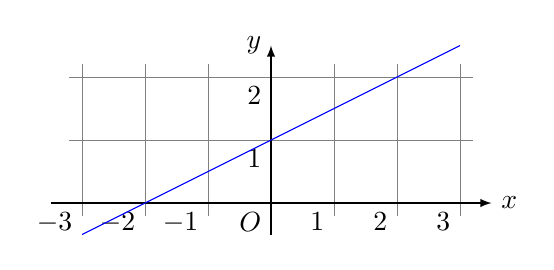
\begin{tikzpicture}[domain={-3:3},scale=0.8]
      \draw[help lines] (-3.2,-0.2) grid (3.2,2.2);
      \node[below left] at (0,0) {$O$};
      \draw[-latex] (-3.5,0) -- (3.5,0) node[right] {$x$};
      \draw[-latex] (0,-0.5) -- (0,2.5) node[left] {$y$};
      \foreach \x in {-3,-2,-1,1,2,3} {
          \node[below left] at (\x,0) {$\x$};
        }
      \foreach \y in {1,2} {
          \node[below left] at (0,\y) {$\y$};
        }

      \draw[blue] plot (\x,0.5*\x+1);
    \end{tikzpicture}
    \caption{$f(x) = 0.5x+1$}
    \label{subfig:fig-test-line}
  \end{subfigure}
  \begin{subfigure}{0.49\textwidth}
    \centering
    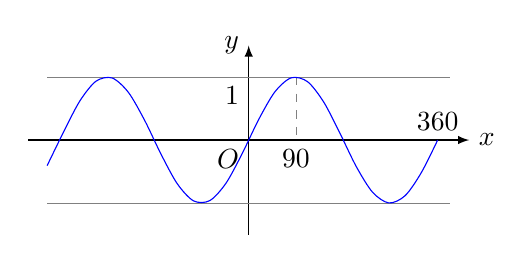
\begin{tikzpicture}[domain={-3.2:3},scale=0.8]
      \node[below left] at (0,0) {$O$};
      \draw[-latex] (-3.5,0) -- (3.5,0) node[right] {$x$};
      \draw[-latex] (0,-1.5) -- (0,1.5) node[left] {$y$};
      \draw[help lines] (-3.2,1) -- (3.2,1) (-3.2,-1) -- (3.2,-1);
      \node[below left] at (0,1) {1};
      \node[above] at (3,0) {$360\degree$};
      \draw[dashed,help lines] (0.75,1)
      -- (0.75,0) node[below,black] {$90\degree$};

      \draw[blue,smooth] plot (\x,{sin(\x*120)});
    \end{tikzpicture}
    \caption{$f(x) = \sin{x}$}
    \label{subfig:fig-test-sine}
  \end{subfigure}
  \caption{函数的图象}
\end{figure}

对于函数$y=f(x)$, 我们比较关注$y$随$x$变化的快慢,
于是我们有\emph{变化率}的概念.
当$x$从$x_1$变化到$x_2$时, 记$x$的变化量$\Delta{x}=x_2-x_1$,
$y$的变化量$\Delta{y}=f(x_2)-f(x_1)$,
我们将
$$
  \dfrac{\Delta{y}}{\Delta{x}} =
  \dfrac{f(x_2)-f(x_1)}{x_2-x_1}
$$
称为函数$f$从$x_1$到$x_2$的平均变化率.
当$x_1,x_2$趋近于$x_0$时 (此时$\Delta{x}$趋近于0),
如果上述的平均变化率趋近于某个常数,
那么我们把这个常数称为函数$f$在$x_0$处的\emph{变化率},
或者瞬时变化率.

\subsection{运动学}

在弹幕制作中我们主要研究点在平面上的运动.
在平面上建立直角坐标系, 点的位置可以由直角坐标$\vec r=(x,y)$确定.
一个点在一个时刻只能有一个位置,
也就是说点的位置是关于时间的函数.
我们把点在$t$时刻的位置记作$\vec r(t)$,
对应的横纵坐标记作$x(t),y(t)$,
用关于$t$的数学表达式来表示位置与时间的函数关系,
形如$x(t) = 3t-2, y(t) = t^2$.

速度是位置$\vec r$随时间$t$的变化率, 我们用
$\vec v=(v_x,v_y)$ (v表示velocity) 来表示速度,
其中$v_x,v_y$是$x,y$随时间的变化率.
类似地, 加速度是速度随时间的变化率,
记作$\vec a=(a_x,a_y)$ (a表示acceleration).

对于点在直线上的运动, 我们可以用位置随时间变化的函数图象来直观展示点的运动情况.
但是对于平面运动, 这样做的效果并不好.
例如, 图\ref{fig:circle-xy-figure}展示了
一个在圆周上运动的点的$x(t)$和$y(t)$图象.
尽管从图象中我们能看出横纵坐标的周期性振动,
但是我们更加关心的运动轨迹(圆周), 运动速度(速度大小不变)
等信息都没有在图象上展现出来.

\begin{figure}[htbp]
  \centering
  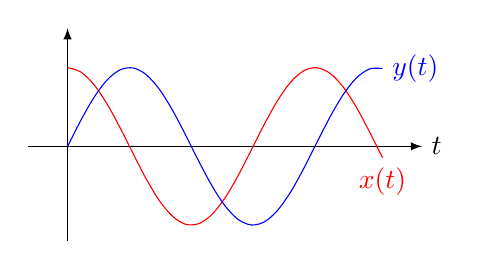
\begin{tikzpicture}
    \draw[-latex] (-0.5,0) -- (4.5,0) node[right] {$t$};
    \draw[-latex] (0,-1.2) -- (0,1.5);

    \draw[smooth,red,domain=0:4] plot (\x,{cos(2*\x r)})
    node[below] {$x(t)$};
    \draw[smooth,blue,domain=0:4] plot (\x,{sin(2*\x r)})
    node[right] {$y(t)$};
  \end{tikzpicture}
  \caption{圆周运动的图象}
  \label{fig:circle-xy-figure}
\end{figure}

在平面运动中, 运动轨迹的形状和长度也是重要的运动属性.
我们把点从$0$时刻到$t$时刻所经过的轨迹长度称为点从$0$到$t$的路程,
记作$s(t)$.

实际上, 速度的大小和方向与运动轨迹和路程有着密切的联系:
\begin{enumerate}[label=(\alph*)]
  \item 速度的大小(被称为速率)等于路程随时间的变化率;
  \item 速度的方向与运动轨迹在对应点处的切线方向共线.
\end{enumerate}

\begin{center}
  \begin{tikzpicture}
    \draw[] (0,0) arc (30:-80:3 and 1)
    node[pos=0.5,dot,sloped] (P) {};
    \draw[->] (P) -- ($(P)!1cm!(P.west)$)
    node[below] {$\vec v$};
  \end{tikzpicture}
\end{center}

在运动学中, 我们认为时间是连续的, 时间间隔可以无限趋近于0,
这是我们用曲线表示运动图象和运动轨迹的基础,
也符合我们对于运动的直观感受.
然而在游戏中, 状态更新和渲染是一帧一帧进行的,
只有整数帧的时刻是有意义的, 最小的时间间隔是1帧.
在这样的体系下, 虽然我们仍然可以定义速度, 加速度等属性, 比如:
(这里用$[t]$是参考了编程语言中数组索引的记法)
\begin{align*}
  \vec v[t] & = \vec r[t] - \vec r[t-1], \\
  \vec a[t] & = \vec v[t] - \vec v[t-1].
\end{align*}

然而由于计算方式不同, 对于同一个运动问题, 两种体系会得到不同的结果.
例如, 下面的伪代码控制一个子弹的速度使得它做匀速圆周运动:

\begin{lstlisting}
无限循环(rot=0, 每轮增加18):
    设置速度(大小=3, 方向=rot)
    等待1帧
\end{lstlisting}

图\ref{fig:discrete-time}展示了子弹的运动情况.
图中的各点是子弹实际运动到的位置, 图中的圆则是运动学
根据初速度和速度方向的变化率推导出的运动轨迹.

\begin{figure}[htbp]
  \centering
  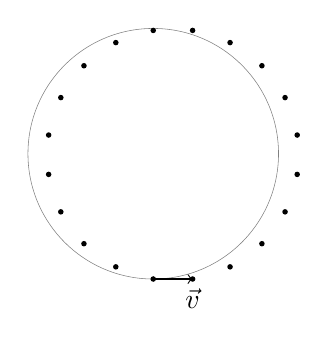
\begin{tikzpicture}[
      declare function={
          v = 0.5;
          w = 18;
          d = (v / w) r;
        }
    ]
    \draw[help lines] (0,0) arc (-90:-90+360:d);
    \fill foreach \i in {0,...,19}
      {++(w*\i:v) circle (1pt)};
    \draw[->] (0,0) -- (v,0) node[below] {$\vec v$};
  \end{tikzpicture}
  \caption{}
  \label{fig:discrete-time}
\end{figure}

尽管有这样的偏差, 本教程还是选择介绍连续时间的运动学而非
间断时间的实际系统. 这是因为连续时间的结论更加简洁,
而且两种体系的偏差对于我们研究的简单运动是可以接受的程度.

\subsection{曲线方程}

数学上通常用\emph{方程}来描述一条曲线.
方程是关于一个或多个变量的等式或不等式, 形如$x^2+2x+1=0$.
如果一组变量值满足该方程, 则称这组值为该方程的一个\emph{解}.
对于平面上的一条曲线和一个(或一组)关于坐标变量$x,y$的方程, 如果
\begin{enumerate}[label=(\alph*)]
  \item 曲线上的每一点, 坐标都满足方程(或方程组);
  \item 满足方程(组)的每一组坐标, 对应点都在曲线上.
\end{enumerate}
那么我们就说该曲线和该方程(组)是对应的.

利用曲线方程, 我们可以把一些几何问题转化为解方程的代数问题.

\begin{example}
  设平面上有一个圆心为原点, 半径为1的圆$C$,
  以及一个端点为$(2,0),(0,1)$的线段$L$.
  我们想求出$C$和$L$的交点.

  我们之后会详细介绍线段和圆的方程, 这里就直接给出结果了.
  圆$C$的方程为$x^2+y^2=1$, 线段$L$的方程为
  $y=-0.5x+1, 0\le{x}\le2$.
  交点应当同时满足$C$和$L$的方程, 于是问题转化为求解下述方程组的解:
  \[
    \begin{cases}
      x^2 + y^2 = 1  \\
      y = -0.5 x + 1 \\
      0 \le x \le 2
    \end{cases}
  \]
  上述方程组的两个解$(0,1)$和$(0.8,0.6)$即为$C$和$L$的两个交点坐标.
\end{example}

根据曲线的特点, 我们有各种不同类型的方程来描述曲线,
以下是几种常见的方程类型.

\subsubsection{函数}

函数$y=f(x)$用横纵坐标之间的函数关系来描述曲线,
这类方程在初中和高中数学十分常用,
在弹幕制作中也是比较好用的.

然而这类方程要求横纵坐标之间必须满足函数关系,
即一个$x$值最多对应一个$y$值.
这使得很多曲线无法用函数描述 (比如圆就不满足函数关系).

$y=f(x)$常用于弹幕的横坐标容易控制的情况.
如果纵坐标更容易控制, 可以考虑$x=g(y)$的形式.

\begin{center}
  \begin{tikzpicture}[
      declare function={
          f(\x) = \x*\x/2;
        }
    ]
    \draw[-latex] (-2.5,0) -- (2.5,0) node[right] {$x$};
    \draw[-latex] (0,-0.5) -- (0,2.5) node[left] {$y$};
    \node[below left] at (0,0) {$O$};
    \draw[domain={-2:2},blue,smooth] plot (\x,{f(\x)})
    node[right] {$y = \dfrac12 x^2$};
  \end{tikzpicture}
\end{center}

\subsubsection{参数方程}

参数方程引入一个参数变量$t$, 用$x,y$和$t$的函数关系描述曲线, 形如
\[
  \begin{cases}
    x = x(t), \\ y = y(t).
  \end{cases}
\]

参数方程在弹幕制作中极为常用, 这有多方面的原因:
\begin{enumerate}
  \item 参数方程的形式与平面运动一致.
        在实际应用中, 参数$t$经常表现为与时间相关,
        甚至直接表示时间,
        有时候参数也会与一些几何属性联系起来.
        总之对于弹幕来说, 参数$t$通常都具有明确的实际含义.
  \item 参数方程能描述的曲线很广泛.
        参数方程兼容函数$y=f(x)$: $x=t, y=f(t)$,
        兼容我们马上要说的极坐标方程$r=r(\theta)$:
        $x=r(t)\cos{t}, y=r(t)\sin{t}$.
        参数方程还能描述很多其他的曲线.
  \item 参数方程容易生成曲线上的点.
        只需要代入$t=t_0$, 就能得到曲线上一点的坐标$(x(t_0),y(t_0))$.
        同时, 由于参数$t$通常有明确的含义,
        我们比较容易根据实际需求去选择曲线上的点.
\end{enumerate}

参数方程也有它的缺点. 如果我们要判断一个点$(x_0,y_0)$是否在曲线上,
就需要判断是否有满足方程$x(t)=x_0,y(t)=y_0$的$t$值,
这是相对困难的.

为了简化表述, 我们可以用向量形式$\vec r=\vec r(t)$表示参数方程.
比如下述参数方程
\begin{align*}
  x & = 13\cos(10t) - 10\cos(13t), \\
  y & = 13\sin(10t) - 10\sin(13t)
\end{align*}
可以记作
\[
\vec r = \braket{13,10t} - \braket{10,13t}.
\]

\begin{center}
  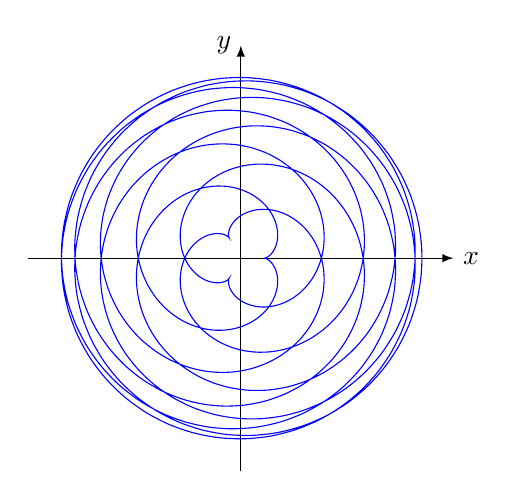
\begin{tikzpicture}[scale=0.1]
    \draw[-latex] (-27,0) -- (27,0) node[right] {$x$};
    \draw[-latex] (0,-27) -- (0,27) node[left] {$y$};
    \draw[domain={0:2*pi},blue,smooth,samples=500] plot (
      {13*cos(10*\x r) - 10*cos(13*\x r)},
      {13*sin(10*\x r) - 10*sin(13*\x r)}
    );
  \end{tikzpicture}
\end{center}

\subsubsection{极坐标方程}

极坐标方程$r=r(\theta)$用极径$t$和极角$\theta$之间的函数关系描述曲线.
尽管极坐标方程能描述的曲线比较少, 但这类曲线在弹幕中还挺常见的,
比如下面的等速螺线, 在各类风车弹中大量出现.

\begin{center}
  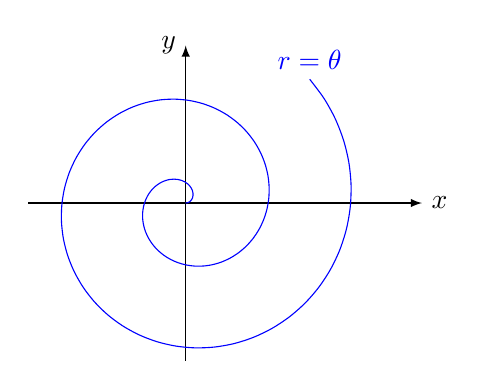
\begin{tikzpicture}
    \draw[-latex] (-2,0) -- (3,0) node[right] {$x$};
    \draw[-latex] (0,-2) -- (0,2) node[left] {$y$};
    \draw[domain={0:4.25*pi},blue,smooth,samples=100] plot (
      {\x*cos(\x r)/6},
      {\x*sin(\x r)/6}
    ) node[above] {$r = \theta$};
  \end{tikzpicture}
\end{center}

\subsubsection{一般方程}

一般方程$F(x,y)=0$用关于横纵坐标的方程表示曲线,
在高中数学中经常使用, 比如圆$x^2+y^2=R^2$, 椭圆
$\dfrac{x^2}{a^2}+\dfrac{y^2}{b^2}=1$等.

一般方程在弹幕制作中用的比较少.
弹幕制作中我们更需要生成曲线上的点,
这在曲线方程中表现为求曲线方程的解,
而求解一般方程很多时候并不容易.
相对地, 一般方程更适合判断某个点是否在曲线上,
只需要把该点坐标代入到方程中判断是否满足方程即可.

\begin{center}
  \begin{tikzpicture}
    \draw[-latex] (-2.5,0) -- (2.5,0) node[right] {$x$};
    \draw[-latex] (0,-1.5) -- (0,1.5) node[left] {$y$};

    \draw[smooth,domain={45:45+360},blue]
    plot ({2*cos(\x)},{1*sin(\x)})
    node[above right] {$\dfrac{x^2}{4}+y^2=1$};
  \end{tikzpicture}
\end{center}
